\section{Objective and Sub-Tasks}
\label{sec:objective}
The main goal of this project is the development of an emergency braking assistant for an electric go-kart that utilizes a radar sensor together with an embedded computing device to detect approaching stationary obstacles and to trigger an emergency braking event when needed.
The test scenario for the emergency braking event consisted of a wall built by 3x3 cubes with a side length of \SI{0.4}{\meter}, resulting in a total size of \SI{1.2}{\meter} by \SI{1.2}{\meter}.
With the wall being approached in a straight line at constant speed from a distance of \SIrange{10}{11}{\meter}, the system should recognize the approaching static object and execute an emergency braking event, effectively stopping the go-kart before it gets into contact with the wall.

\begin{figure}[!htbp]
    \centering
    %\resizebox{0.48\textwidth}{!}{
        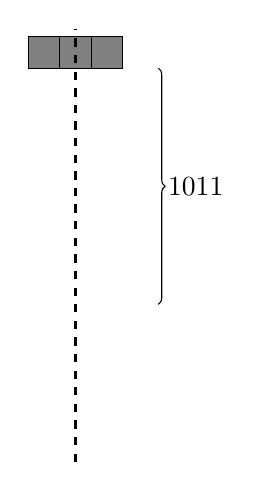
\begin{tikzpicture}
            \gokart{0}{0}{0}
        
            %Wall (three cubes)
            \draw[fill=gray] (-0.6,3) rectangle (-0.2,3.4);
            \draw[fill=gray] (-0.2,3) rectangle (0.2,3.4);
            \draw[fill=gray] (0.2,3) rectangle (0.6,3.4);
        
            %Dashed line from go-kart to wall
            \draw[dashed, thick] (0,-2) -- (0,3.5);

            \draw [decorate, decoration = {brace, raise=10pt}] (0.7,3) -- (0.7, 0) node[pos=0.5,right=10pt,black]{\SIrange{10}{11}{\meter}};
        \end{tikzpicture}
    %}
    \caption{Test scenario}
    \label{fig:test_scenario}
\end{figure}
\par
%% [14/03/2025] Luis: Rework so it does not sound so "school project"
%% ---------------------------------------
A Ninebot Go-kart PRO electric go-kart was selected as the test vehicle for this implementation, equipped with a Texas Instruments IWR6843AOPEVM development board, featuring the IWR6843AOP mmWave radar sensor, for data acquisition and sensing tasks.
% Since the project was conducted in form of a one-semester research seminar and the associated lab already provided those resources, a Ninebot Go-kart PRO electric go-kart was used as the project's vehicle and a IWR6843AOPEVM development board from Texas Instruments, featuring a IWR6843AOP radar sensor, for the sensing part.
\newpage

\subsection{Sub-Tasks}

The main objective, together with the given boundary conditions in form of the given test scenario and the provided electric go-kart and radar sensor, implied several practical sub-tasks:
\begin{itemize}
    \item Finding ways to manipulate the go-kart’s controller for performing the braking operation.
    \item Interfacing the radar sensor and finding a suitable configuration.
    \item Choosing an embedded computation device.
    \item Developing and implementing a live processing pipeline.
    \item Joining the individual parts and testing the system.
\end{itemize}
As the usage of a generic electric go-kart required its reverse engineering for finding possible ways of interfacing the go-kart's braking system and those findings significantly constrained the solution space of the other sub-tasks, the tasks' ordering was kept and the whole project followed an agile approach.